\documentclass[xetex,serif, onlymath]{beamer}

\usepackage[T1]{fontenc}
\usepackage[usefilenames,% Important for XeLaTeX
  DefaultFeatures={Ligatures=Common}]{plex-otf} %
\renewcommand*\familydefault{\sfdefault} %% Only if the base font of the document is to be sans serif

\usetheme{hsr}

\title{\textrm{\LaTeX} Workshop}
\author[NaoPross]{Naoki Pross \texttt{<npross@hsr.ch>}}
\date{\today}

\institute[HSR]{Hochschule f\"ur Technik Rapperswil}
%\logo{
\includegraphics[width=3cm]{figs/hsr-logo}}

\AtBeginSection[]
{
  \begin{frame}
    \frametitle{Table of Contents}
    \tableofcontents[currentsection]
  \end{frame}
}


\begin{document}
\begin{frame}
\maketitle
\end{frame}

\begin{frame}{Goal: Learn to typeset something like this}
	\begin{center}
		\vspace{1cm}
		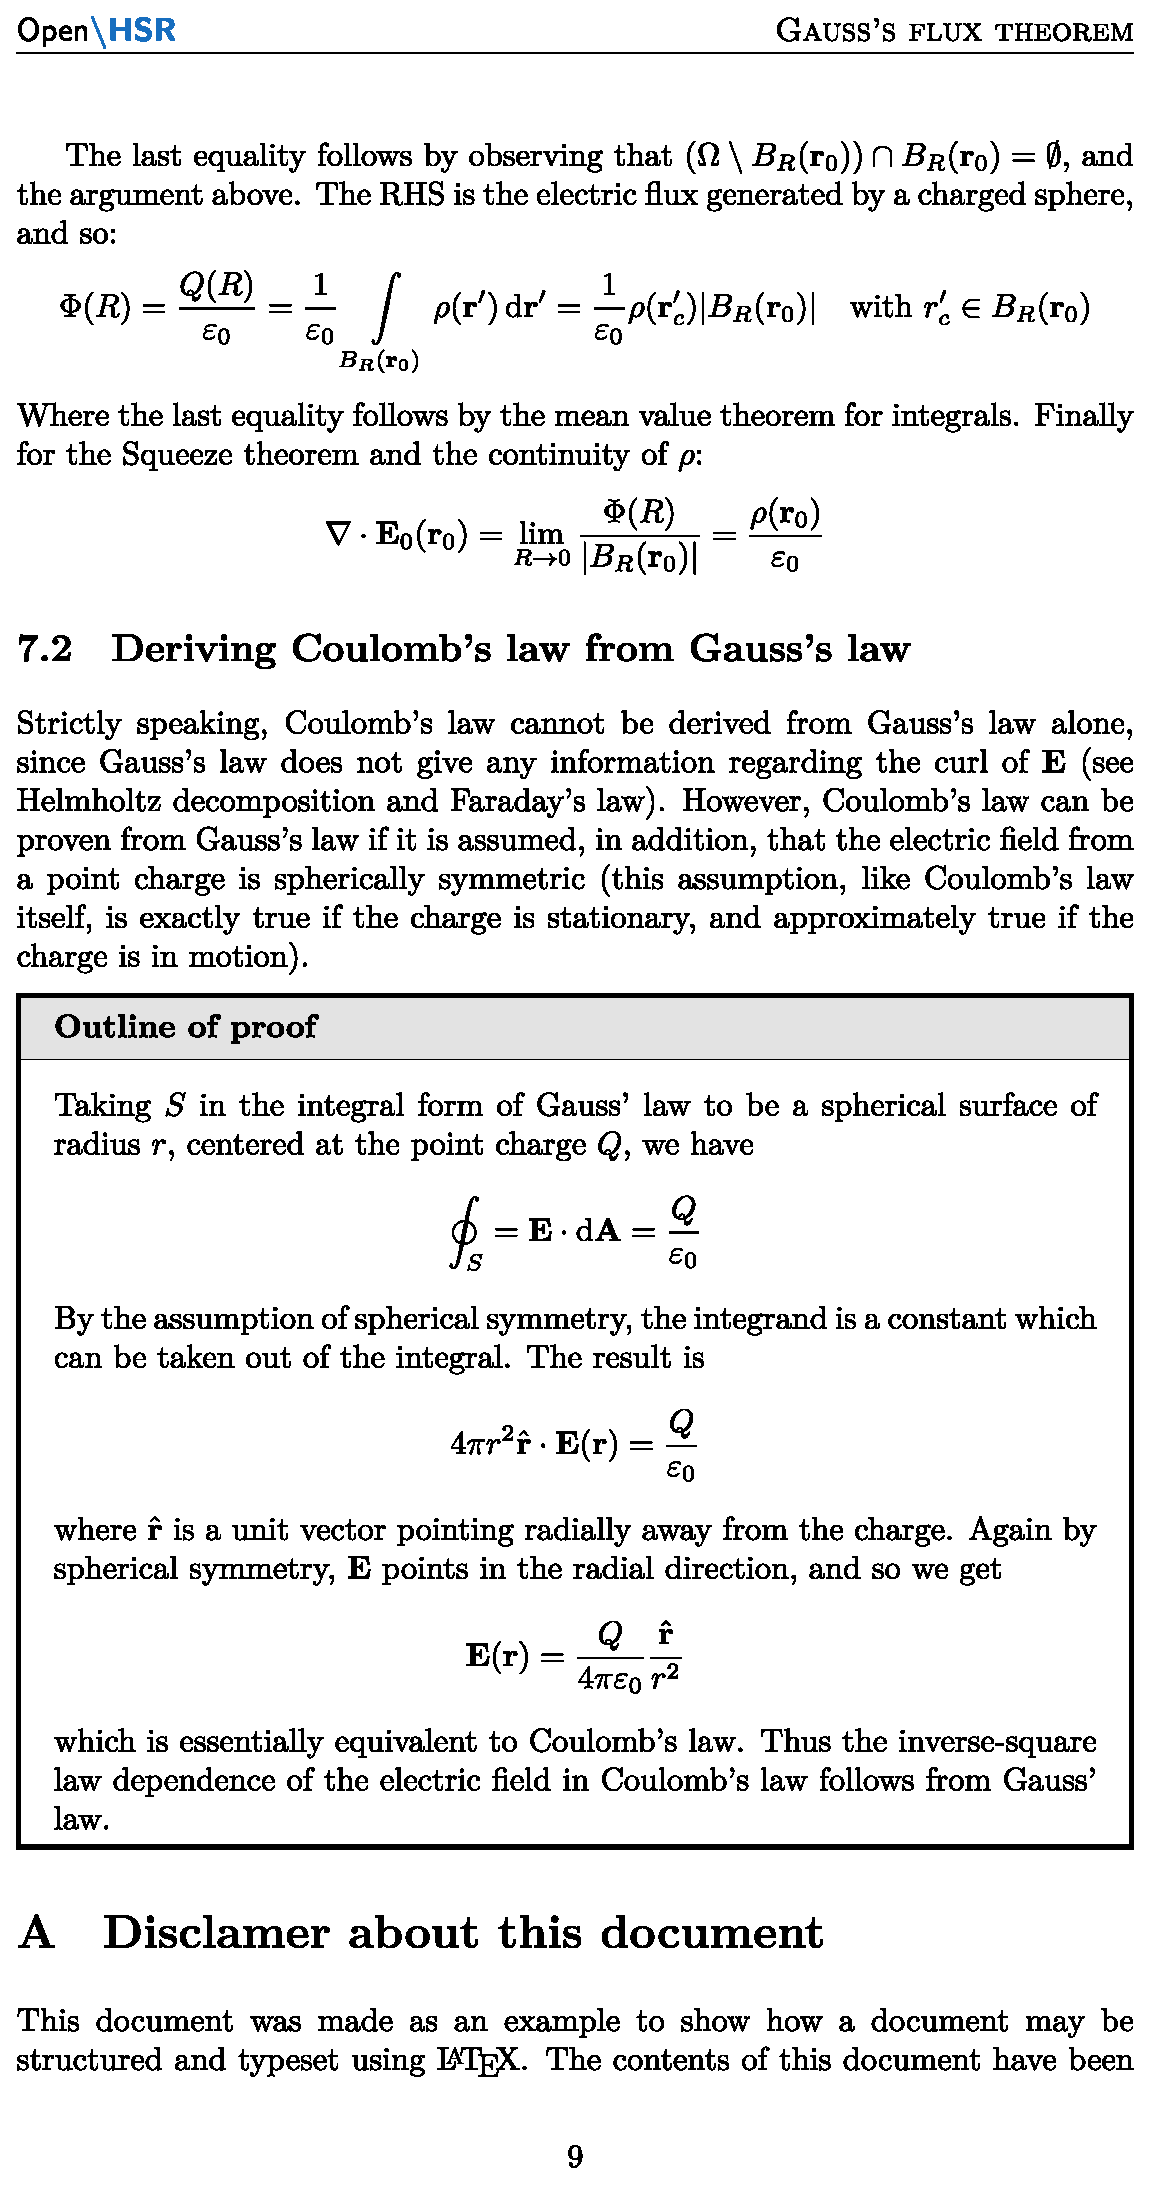
\includegraphics[width=.8\linewidth]{figs/gauss-flux}
	\end{center}
\end{frame}

\section{Introduction}

\begin{frame}{What is Typesetting}
\end{frame}

\begin{frame}{History \& \textrm{\LaTeX}}
\end{frame}

\section{Fundamentals}
\begin{frame}{Source code spacing}
\end{frame}

\begin{frame}{Special characters}
\end{frame}

\begin{frame}{Commands}
\end{frame}

\begin{frame}{Environments}
\end{frame}

\begin{frame}{Document structure}
\end{frame}

\begin{frame}{Spacing and newlines}
\end{frame}

\section{Basics}
\begin{frame}{Emphasis, Bold, Italic}
\end{frame}

\begin{frame}{Lists}
\end{frame}

\begin{frame}{Tables}
\end{frame}

\begin{frame}{Figures (floats)}
\end{frame}

\begin{frame}{Cross-References}
\end{frame}

\section{Mathematics}
\begin{frame}{Math environments}
\end{frame}

\begin{frame}{Math symbols and fonts}
\end{frame}

\begin{frame}{Equations}
\end{frame}

\begin{frame}{Spacing in math mode}
\end{frame}

\section{Bibliography management}
\begin{frame}{TheBibliography}
\end{frame}

\begin{frame}{External bibliography}
\end{frame}

\section{Extras}
\begin{frame}{Source code listings}
\end{frame}

\begin{frame}{Plots}
\end{frame}

\begin{frame}{TikZ}
\end{frame}

\end{document}